\documentclass[a4paper]{article}
\title{TLE Scenario Generator}
\author{SolarLiner}

\usepackage{graphicx}
\usepackage{hyperref}
\usepackage{booktabs}

\usepackage{geometry}
  \geometry{
	a4paper,
	left=0.8in,
	right=0.8in,
	top=1in,
  }
\usepackage[default]{lato}
\usepackage[T1]{fontenc}
\usepackage{sourcecodepro}

\begin{document}
	\pagenumbering{gobble}
	\maketitle
	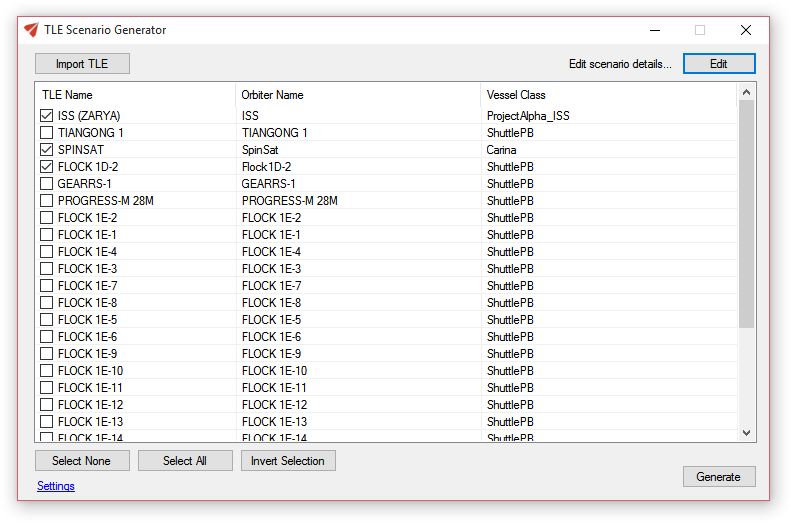
\includegraphics[width=\linewidth]{mainwindow.png} 
	This software is released in a beta state, which means that bugs are to be expected, and may be reported to either Orbiter-Forum, or to the repository on GitHub.
	\newpage
	\tableofcontents
	\newpage
	\pagenumbering{arabic}
	
	\part{Introduction}
	The Two-Line element set, abbreviated to TLE, is a data format encoding orbital elements of an Earth-orbiting object.\\
	Data is written as two lines of 80 ASCII-encoded characters, preceded by an optional title line.
	
	Currently the United States Air Forces tracks all non-classified objects, and makes them available on \href{https://www.space-track.org/}{Space Track}. Another site which doesn't require an account is \href{https://celestrak.com/}{Celestrack}, maintained by NORAD, which hosts the file used by default in this application.
	\section{Structure of a TLE set}
		Each line begins with its line number and ends with a check sum modulo of 10.\\
		The first line holds object identification data, as well as aerodynamic constants used by simplified perturbations models (unused in this application as Orbiter will use the loaded vessels to compute drag loss).
		
		Considering this TLE set:\\
		\texttt{ISS (ZARYA)\\
1 25544U 98067A   08264.51782528 -.00002182  00000-0 -11606-4 0  2927\\
2 25544  51.6416 247.4627 0006703 130.5360 325.0288 15.72125391563537}
		\begin{table}[h!]
			\centering
			\caption{Line 1 of a TLE set}
			\begin{tabular}{lll}
				\textbf{Column Number} & \textbf{Description}                                                             & \textbf{Example} \\ \midrule
				1                        & Line Number of Element Data                                                      & 1                \\ \midrule
				03-07                    & Satellite Number                                                                 & 25544            \\ \midrule
				8                        & Classification (U=Unclassified)                                                  & U                \\ \midrule
				10-11                    & International Designator (Last two digits of launch year)                        & 98               \\ \midrule
				12-14                    & International Designator (Launch number of the year)                             & 067              \\ \midrule
				15-17                    & International Designator (Piece of the launch)                                   & A                \\ \midrule
				19-20                    & Epoch Year (Last two digits of year)                                             & 8                \\ \midrule
				21-32                    & Epoch (Day of the year and fractional portion of the day)                        & 264.51782528     \\ \midrule
				34-43                    & First Time Derivative of the Mean Motion                                         & -.00002182       \\ \midrule
				45-52                    & Second Time Derivative of Mean Motion (decimal point assumed)                    & 00000-0          \\ \midrule
				54-61                    & BSTAR drag term (decimal point assumed)                                          & -11606-4         \\ \midrule
				63                       & Ephemeris type                                                                   & 0                \\ \midrule
				65-68                    & Element number                                                                   & 292              \\ \midrule
				69                       & Checksum (Modulo 10) & 7 \\ \bottomrule
			\end{tabular}
		\end{table}
		
		\begin{table}[h!]
			\centering
			\caption{Line 2 of a TLE set}
			\begin{tabular}{lll}
				\textbf{"Column Number"} & \textbf{Description}                                & \textbf{Example} \\ \midrule
				1                        & Line Number of Element Data                         & 2                \\ \midrule
				03-07                    & Satellite Number                                    & 25544            \\ \midrule
				09-16                    & Inclination {[}Degrees{]}                           & 51.6416          \\ \midrule
				18-25                    & Right Ascension of the Ascending Node {[}Degrees{]} & 247.4627         \\ \midrule
				27-33                    & Eccentricity (decimal point assumed)                & 0006703          \\ \midrule
				35-42                    & Argument of Perigee {[}Degrees{]}                   & 130.5360         \\ \midrule
				44-51                    & Mean Anomaly {[}Degrees{]}                          & 325.0288         \\ \midrule
				53-63                    & Mean Motion {[}Revs per day{]}                      & 15.72125391      \\ \midrule
				64-68                    & Revolution number at epoch {[}Revs{]}               & 56353            \\ \midrule
				69                       & Checksum (Modulo 10)                                & 7                \\ \bottomrule
			\end{tabular}
		\end{table}
		\newpage
		\section{TLEs and Orbiter}
		Two-Line Elements can be a very valuable tool for reality-based scenarii making, to recreate existing missions or set up a fictional mission based on a real environment. It is also a quick way of adding vessels to a scenario, filling up the otherwise empty Low Earth Orbit.
		
		Currently, using the ISS' TLE set as benchmark, the application generates a scenario that is true to ISS position at $\pm$ 100 km, and is in advance by $\pm$ 10 seconds in its orbit. Possible reasons to such differences will be covered later.\\
		As a result, it is possible, to a certain degree, to visualize object trajectories interactively.
		
	\newpage
	\part{Application Quickstart}
		\section{Loading a TLE resource}
			The first step to converting TLE data into an Orbiter scenario is to import the resource by providing its URL. Click on the 'Import' button on the top left of the application and paste the link. By default is entered the Station sets from the Celestrak website, allowing you to quickly get the ISS' orbital info.
			
			Once imported, the main window will display a list of objects as parsed from the file. From there you can check or uncheck imported objects; only checked objects will be included in the generated scenario.\\
			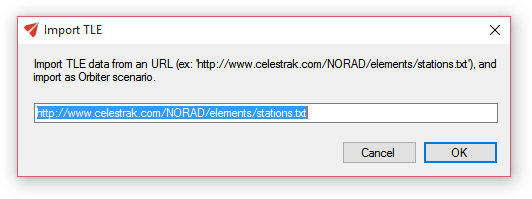
\includegraphics[scale=1]{import_tle.png}
			
		\section{Editing vessel details}
			By double clicking on any entry, you will be able to edit the Orbiter name of the object, its vessel class, and in future versions, its scenario details (fuel, attachments, dock info, etc.). Are also displayed the TLE lines, and its TLE name, if any.\\
			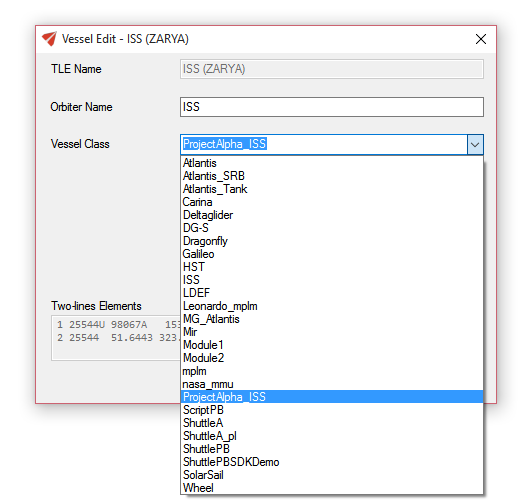
\includegraphics[scale=1]{vessel_edit.png}
			
		\section{Editing scenario properties}
			Once you have edited and checked all the objects you wanted in your scenario, you can then edit the scenario description and date using the top right button 'edit'.\\
			From there you can edit the name, description and date of your scenario.\\
			Leaving 'Always use system time' checked will omit the MJD entry in the scenario, forcing Orbiter to run the simulation with the current system time, allowing for observations in more or less real time.\\
			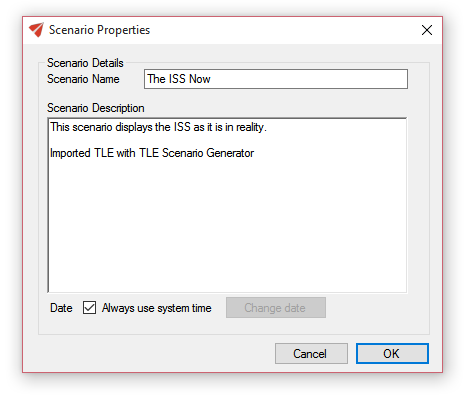
\includegraphics[scale=1]{scn_properties.png}
			
		\section{Generating the scenario}
			Hit the bottom-right-most button to generate and save the scenario. You can then launch it with Orbiter, or open it and modify it in greater lengths than this tool was created for.\\
			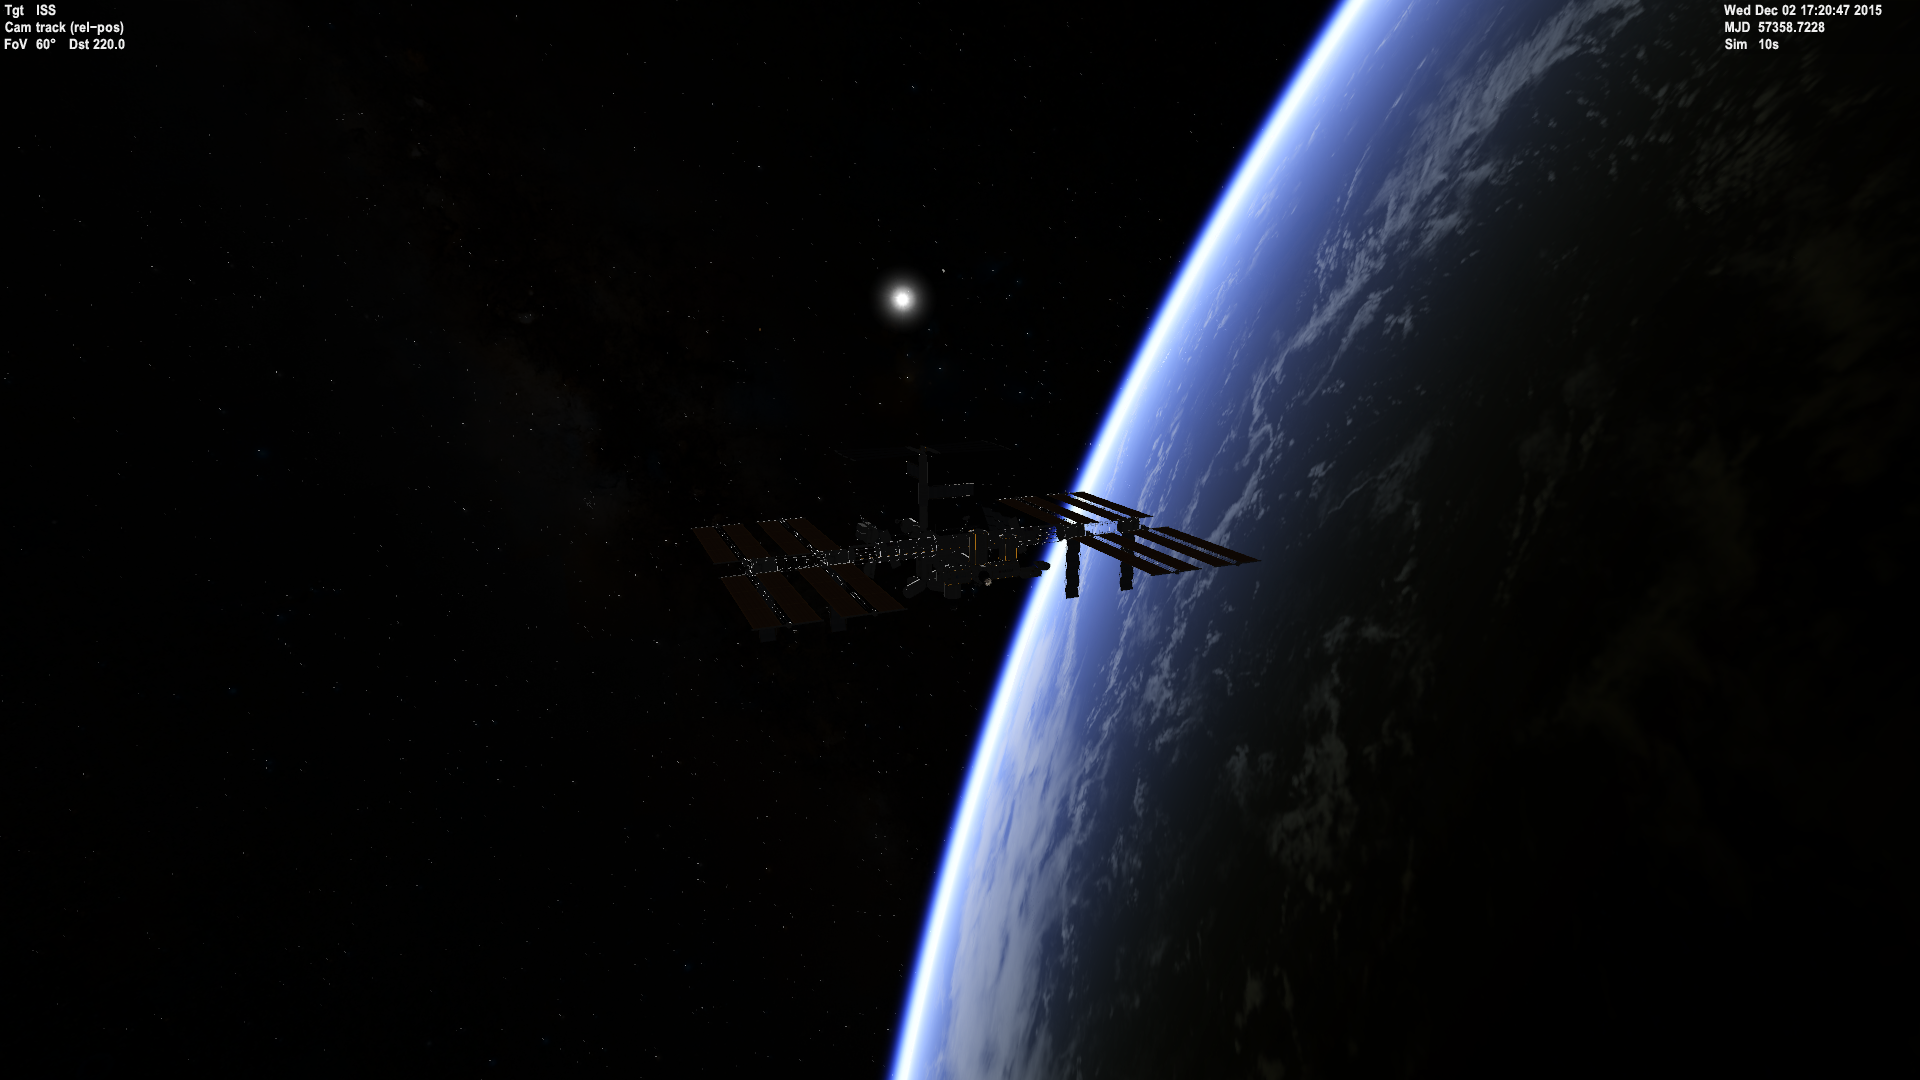
\includegraphics[width=\linewidth]{scn_result.png}
			
	\newpage
	\part{Appendix}
		\section{The settings}
			On the bottom-left of the window features a link to the programs' settings, allowing you to choose your language and specify the path to your Orbiter directory.\\
			This allows the application to search for vessels in its Config folder, and populate the auto-completion feature of the Vessel Edit window.\\
			\includegraphics[scale=1]{../bin/Debug/settings.png} 
			
		\section{On the differences between reality and simulation}
			While the conversion algorithm to extract and convert TLE data into orbital element would be the main cause, I suspect Orbiter to use a 'on-rails' propagation of objects from those elements, up to the starting date of the scenario. In this case, perturbations are simply ignored, and the object will follow its orbital path as if it was evolving in a true vacuum. But atmospheric drag at altitudes this high shouldn't lead to a 50 to 100 km difference.
			
	\newpage
	\part{End notes}
		The link to the GitHub repository can be found here: \url{https://github.com/SolarLiner/TLEOrbiter}.\\
		Orbiter Forum thread is not yet created - it will be added onto the GitHub page, and here in another version.
		
		\textbf{Thanks to} Face for his bug hunting work and patches, I would have never have known ;)
\end{document}
